% Options for packages loaded elsewhere
\PassOptionsToPackage{unicode}{hyperref}
\PassOptionsToPackage{hyphens}{url}
%
\documentclass[
]{article}
\usepackage{amsmath,amssymb}
\usepackage{lmodern}
\usepackage{iftex}
\ifPDFTeX
  \usepackage[T1]{fontenc}
  \usepackage[utf8]{inputenc}
  \usepackage{textcomp} % provide euro and other symbols
\else % if luatex or xetex
  \usepackage{unicode-math}
  \defaultfontfeatures{Scale=MatchLowercase}
  \defaultfontfeatures[\rmfamily]{Ligatures=TeX,Scale=1}
\fi
% Use upquote if available, for straight quotes in verbatim environments
\IfFileExists{upquote.sty}{\usepackage{upquote}}{}
\IfFileExists{microtype.sty}{% use microtype if available
  \usepackage[]{microtype}
  \UseMicrotypeSet[protrusion]{basicmath} % disable protrusion for tt fonts
}{}
\makeatletter
\@ifundefined{KOMAClassName}{% if non-KOMA class
  \IfFileExists{parskip.sty}{%
    \usepackage{parskip}
  }{% else
    \setlength{\parindent}{0pt}
    \setlength{\parskip}{6pt plus 2pt minus 1pt}}
}{% if KOMA class
  \KOMAoptions{parskip=half}}
\makeatother
\usepackage{xcolor}
\IfFileExists{xurl.sty}{\usepackage{xurl}}{} % add URL line breaks if available
\IfFileExists{bookmark.sty}{\usepackage{bookmark}}{\usepackage{hyperref}}
\hypersetup{
  pdftitle={COVID-19 Vaccine Equity Analysis (DRAFT)},
  pdfauthor={Amy Johnson, PhD \textbar{} C. Scott Smith, PhD AICP},
  hidelinks,
  pdfcreator={LaTeX via pandoc}}
\urlstyle{same} % disable monospaced font for URLs
\usepackage[margin=1in]{geometry}
\usepackage{longtable,booktabs,array}
\usepackage{calc} % for calculating minipage widths
% Correct order of tables after \paragraph or \subparagraph
\usepackage{etoolbox}
\makeatletter
\patchcmd\longtable{\par}{\if@noskipsec\mbox{}\fi\par}{}{}
\makeatother
% Allow footnotes in longtable head/foot
\IfFileExists{footnotehyper.sty}{\usepackage{footnotehyper}}{\usepackage{footnote}}
\makesavenoteenv{longtable}
\usepackage{graphicx}
\makeatletter
\def\maxwidth{\ifdim\Gin@nat@width>\linewidth\linewidth\else\Gin@nat@width\fi}
\def\maxheight{\ifdim\Gin@nat@height>\textheight\textheight\else\Gin@nat@height\fi}
\makeatother
% Scale images if necessary, so that they will not overflow the page
% margins by default, and it is still possible to overwrite the defaults
% using explicit options in \includegraphics[width, height, ...]{}
\setkeys{Gin}{width=\maxwidth,height=\maxheight,keepaspectratio}
% Set default figure placement to htbp
\makeatletter
\def\fps@figure{htbp}
\makeatother
\setlength{\emergencystretch}{3em} % prevent overfull lines
\providecommand{\tightlist}{%
  \setlength{\itemsep}{0pt}\setlength{\parskip}{0pt}}
\setcounter{secnumdepth}{5}
\usepackage{booktabs}
\usepackage{longtable}
\usepackage{array}
\usepackage{multirow}
\usepackage{wrapfig}
\usepackage{float}
\usepackage{colortbl}
\usepackage{pdflscape}
\usepackage{tabu}
\usepackage{threeparttable}
\usepackage{threeparttablex}
\usepackage[normalem]{ulem}
\usepackage{makecell}
\usepackage{xcolor}
\ifLuaTeX
  \usepackage{selnolig}  % disable illegal ligatures
\fi

\title{COVID-19 Vaccine Equity Analysis (DRAFT)}
\author{Amy Johnson, PhD \textbar{} C. Scott Smith, PhD AICP}
\date{Last updated 4/21/2021}

\begin{document}
\maketitle

{
\setcounter{tocdepth}{2}
\tableofcontents
}
\hypertarget{background}{%
\section{Background}\label{background}}

The illness caused by Severe Acute Respiratory Syndrome Coronavirus-2 (SARS-CoV-2), coronavirus disease (COVID-19), was declared a pandemic by the World Health Organization in March 2020. In absence of a cure and natural immunity, more than 500,000 Americans have died of COVID-19 and far more have been impacted by the disease.

However, the distribution of the disease is not uniform across the American population, but rather the burden of COVID-19 has disproportionately impacted racial and ethnic minorities demonstrating the effects of social determinants of health, neighborhood traits, and the distribution of underlying comorbidities {[}ADD CITATIONS{]}. Racial/ethnic minority populations in urban settings are often employed in service occupations that prevent work-from-home and physical distancing. Further, crowded, multi-generational households, older housing stock, and substandard air quality also contribute to the increased rates of COVID-19 among racial/ethnic minority communities. Finally, racial/ethnic minority populations experience a disproportionate burden of comorbidities that impact the severity of COVID-19 (e.g., diabetes, cardiovascular disease, asthma, obesity). Identifying characteristics that are associated with increased COVID-19 risk, even if they are not causally related, can assist in prioritizing communities with high need for testing and vaccination to mitigate the continued impact of COVID-19.

According to the DePaul University Chicago COVID-19 Community Health Equity dashboard which sources data from local reporting, the city of Chicago has recorded 244,230 positive COVID-19 cases from March 13, 2020 through April 21, 2021 resulting in 4,984 deaths. Despite representing 29\% and 28.8\% of the city's total population, Black and Latinx populations represented 38.5\% and 33.4\% of deaths from COVID-19 respectively. Two highly effective COVID-19 vaccines were approved for emergency use in the United States in December 2020 and a third\ldots{} As COVID-19 vaccination is one of the best strategies to control spread and reduce morbidity and mortality, rapid and equitable dissemination is required. Public health officials need to plan strategically to prioritize the allocation of vaccine to the groups most in need including those disproportionately impacted by COVID-19.

\hypertarget{covid-19-burden-in-chicago}{%
\subsection{COVID-19 Burden in Chicago}\label{covid-19-burden-in-chicago}}

The Chicago COVID-19 Community Vulnerability Index (CCVI) was adapted and modified based on the CDC Social Vulnerability Index. The Chicago CCVI identifies communities that are uniquely vulnerable to barriers to COVID-19 vaccine uptake via a ranking of a combination of ten components (risk factors and COVID-19 burden) that are synthesized into a single composite score. Community areas that received high CCVI scores had the highest mobility during COVID-19, low socioeconomic status, high rates of COVID-19 hospital admission, and high rates of COVID-19 mortality. Fifteen community areas in Chicago made up the top quintile and corresponded to 7 majority Latinx and 8 majority Black community areas. As COVID-19 vaccines are in limited supply, allocation with a focus on communities most impacted is imperative for equitable and effective control.

On January 25, 2021, Chicago Mayor Lori Lightfoot and the Chicago Department of Public Health announced its Protect Chicago Plus (PCP) vaccination program, which is designed to ensure equitable vaccine access for communities that experienced the highest CCVI. The plan identified 15 high-need communities which ranked highest according to the city's CCVI, increasing vaccine allocation in these areas and expanding eligibility to all residents 18 and over. The leveraged community stakeholders to reduce barriers to vaccine access via call-in lines, strike teams, mobile clinics, homebound distribution and other strategies to improve vaccine availability and acceptability.

\hypertarget{research-questions}{%
\subsection{Research Questions}\label{research-questions}}

This study provides an overview of Chicago's COVID-19 vaccine distribution over a four-month period with a particular focus on evaluating whether or not improvements were made in the uptake of vaccine among the city's most vulnerable populations after implementation of its targeted distribution plan. Specifically, this research aims to respond to two research questions:

\begin{enumerate}
\def\labelenumi{(\arabic{enumi})}
\item
  How do first-dose COVID-19 vaccination administrations differ across Chicago communities with different race, ethnic, socioeconomic and CCVI characteristics?
\item
  To what extent have vaccination distribution strategies mitigated disparities in vaccination rates, especially in neighborhoods targeted in the city's Protect Chicago Plus program?
\end{enumerate}

\hypertarget{methodology}{%
\section{Methodology}\label{methodology}}

A series of chi-square analyses were employed to evaluate disparities in vaccination rates across communities categorized by dominant race and ethnic group, poverty status and relative CCVI. Multiple interrupted time series analyses (ITS) were then implemented to evaluate the impact of the city's PCP program on different measures of vaccination coverage and disparity, pre- and post-intervention. ITS was the preferred analytic framework because it required fewer controls, allowing for general inferences to be made about intervention efficacy with two independent variables - time and program start date.

\hypertarget{data}{%
\subsection{Data}\label{data}}

To carry out the above analyses, we rely on publicly available data including:

\begin{enumerate}
\def\labelenumi{(\arabic{enumi})}
\item
  socioeconomic data including race, ethnicity, socioeconomic status and age composition from the US Census Bureau's American Community Survey (ACS), 2015 to 2019 5-year estimates;
\item
  daily first dose COVID-19 vaccination counts from the City of Chicago's data portal; and
\item
  press releases from the City of Chicago and related media reports concerning the geographic scope, roll-out and overall implementation of the city's Protect Chicago Plus vaccination program.
\end{enumerate}

\hypertarget{covid-19-vaccination-disparities-in-chicago}{%
\subsubsection{COVID-19 Vaccination Disparities in Chicago}\label{covid-19-vaccination-disparities-in-chicago}}

\begin{table}

\caption{\label{tab:vaccinations-by-race}First Dose COVID-19 Vaccination Rates by Dominant Community Race and Ethnic Group, 12/15/2020 to 4/19/2021}
\centering
\begin{tabular}[t]{lllr}
\toprule
Dominant Group & First Doses & Pop 18+ & First Dose Rate (\%)\\
\midrule
ASIAN & 22,727 & 46,368 & 49.0\\
BLACK & 234,630 & 608,511 & 38.6\\
LATINX & 256,308 & 484,310 & 52.9\\
WHITE & 587,574 & 1,046,198 & 56.2\\
\bottomrule
\end{tabular}
\end{table}

\begin{table}

\caption{\label{tab:vaccinations-by-poverty}First Dose COVID-19 Vaccination Rates by Poverty Rate Quintile, 12/15/2020 to 4/19/2021}
\centering
\begin{tabular}[t]{rrllr}
\toprule
Poverty Quintile & Mean Poverty Rate & First Doses & Pop 18+ & First Dose Rate (\%)\\
\midrule
1 & 6.84 & 183,664 & 339,176 & 54.2\\
2 & 10.10 & 263,689 & 467,498 & 56.4\\
3 & 17.10 & 327,987 & 590,881 & 55.5\\
4 & 23.60 & 190,973 & 439,189 & 43.5\\
5 & 33.30 & 134,926 & 348,643 & 38.7\\
\bottomrule
\end{tabular}
\end{table}

\begin{table}

\caption{\label{tab:vaccinations-by-pcp}First Dose COVID-19 Vaccination Rates by PCP Community Category, 12/15/2020 to 4/19/2021}
\centering
\begin{tabular}[t]{lllr}
\toprule
PCP Neighborhood & First Doses & Pop 18+ & First Dose Rate (\%)\\
\midrule
NO & 852,523 & 1,632,972 & 52.2\\
YES & 248,716 & 552,415 & 45.0\\
\bottomrule
\end{tabular}
\end{table}

\hypertarget{analysis}{%
\subsection{Analysis}\label{analysis}}

Two-way contingency tables were created to represent daily cumulative first dose COVID-19 vaccination coverage rates by zip code category from December 29, 2020 (two weeks after the first COVID-19 vaccination dose was administered in the city) to April 19, 2021. Zip codes were categorized, ``yes'' and ``no'', by whether they were or were not targeted in the city's PCP program.

For each contingency table, a Pearson chi-squared test was carried out to detect statistically significant differences between vaccination coverage rates across the two categories of communities; with the null hypotheses being that no association exists. Each of these tests yielded a significant p-value, indicating that PCP participation and corresponding vaccination rates are associated throughout the entire study period although variations in the magnitude of these associations change over time.

Figure 1 plots both the standardized and non-standardized residuals from the chi-square tests. Values positioned above the horizontal axis (i.e., greater than 0) indicate vaccination rates that are significantly greater than would be expected if the null hypothesis were true, whereas values positioned below the horizontal axis indicate rates that are significantly lower than would be expected. The plot clearly shows that, when evaluated collectively, communities that rank highest with respect to COVID-19 vulnerability, also underperform with respect to COVID-19 vaccination coverage. However, this gap narrowed in early February (indicated with black vertical line) after the initial roll-out of the PCP vaccination program before widening again in late March as vaccine eligibility expanded to the broader population.

\begin{figure}
\centering
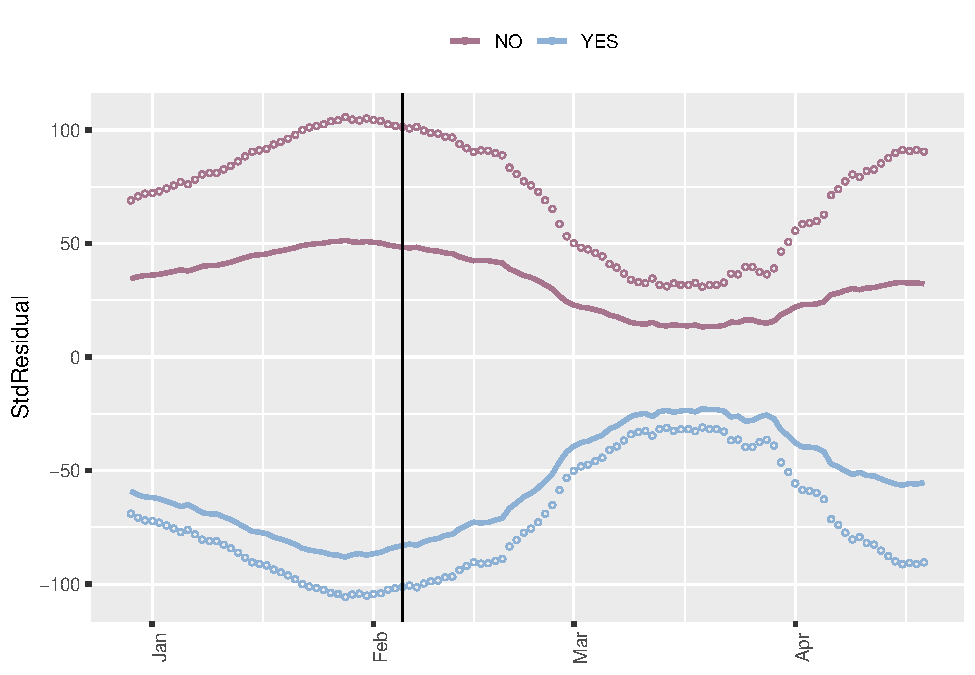
\includegraphics{VaccineEquityInChicago_20210410_files/figure-latex/chi-square-analysis-1.pdf}
\caption{\label{fig:chi-square-analysis}Standardized and Non-Standardized Residuals of Chi-Square Analyses Comparing Daily Cumulative First Dose COVID-19 Vaccination Counts for Communities Inside (YES) and Outside (NO) PCP Target Area}
\end{figure}

\begin{figure}
\centering
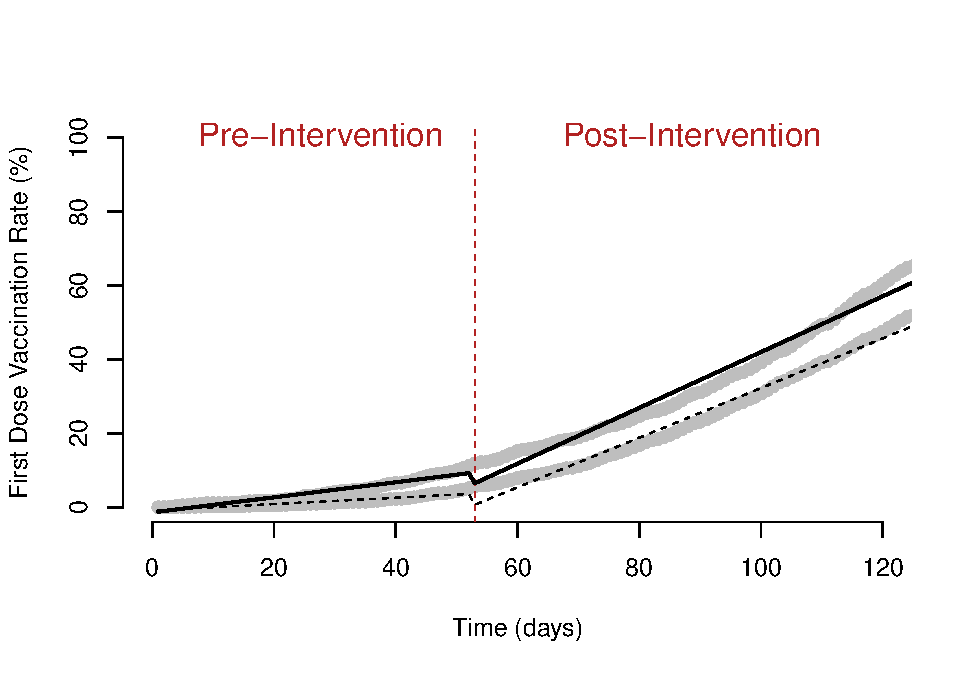
\includegraphics{VaccineEquityInChicago_20210410_files/figure-latex/ITS-plot_pcp-1.pdf}
\caption{(\#fig:ITS-plot\_pcp)Interrupted Time Series (ITS) Analysis of Cumulative First-Dose COVID-19 Vaccination Rates, Pre- and Post-Rollout of the Protect Chicago Plus Program by Community Category}
\end{figure}

\begin{table}[!htbp] \centering 
  \caption{} 
  \label{} 
\begin{tabular}{@{\extracolsep{5pt}}lc} 
\\[-1.8ex]\hline 
\hline \\[-1.8ex] 
 & \multicolumn{1}{c}{\textit{Dependent variable:}} \\ 
\cline{2-2} 
\\[-1.8ex] & COVID-19 First Vaccination Rate \\ 
 & Model results \\ 
\hline \\[-1.8ex] 
 Time & 0.20$^{***}$ \\ 
  & (0.02) \\ 
  & \\ 
 PCP & $-$3.46$^{***}$ \\ 
  & (0.80) \\ 
  & \\ 
 Time Since PCP & 0.55$^{***}$ \\ 
  & (0.02) \\ 
  & \\ 
 Constant & $-$1.41$^{**}$ \\ 
  & (0.63) \\ 
  & \\ 
\hline \\[-1.8ex] 
\hline 
\hline \\[-1.8ex] 
\textit{Note:}  & \multicolumn{1}{r}{$^{*}$p$<$0.1; $^{**}$p$<$0.05; $^{***}$p$<$0.01} \\ 
\end{tabular} 
\end{table}

\begin{figure}
\centering
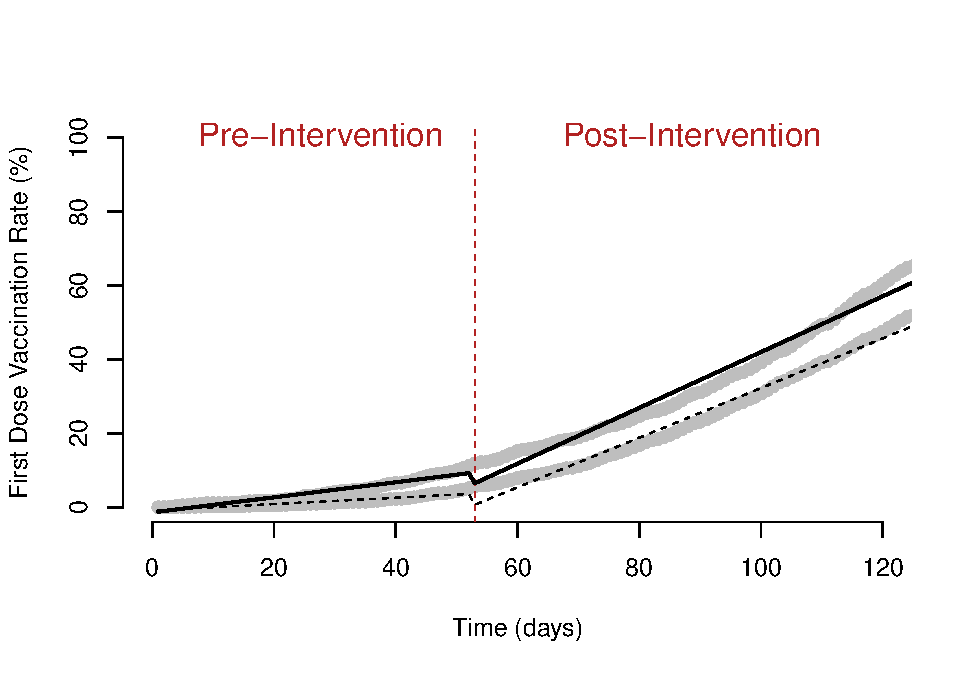
\includegraphics{VaccineEquityInChicago_20210410_files/figure-latex/ITS-plot_pcp_zipspecific-1.pdf}
\caption{(\#fig:ITS-plot\_pcp\_zipspecific)Interrupted Time Series (ITS) Analysis of Cumulative First-Dose COVID-19 Vaccination Rates, Pre- and Post-Rollout of the Protect Chicago Plus Program by Community Category}
\end{figure}

\end{document}
